\documentclass[11pt]{article}


\usepackage[sort]{natbib}
\usepackage{bm,amsmath,bbm,amsfonts,nicefrac,latexsym,amsmath,amsfonts,amsbsy,amscd,amsxtra,amsgen,amsopn,bbm,amsthm,amssymb,graphicx}
\usepackage{wrapfig, caption, subcaption}
\usepackage{fancyhdr, tabularx}
\usepackage[margin=1.0in]{geometry}
\bibliographystyle{abbrvnat}
%\usepackage[section]{placeins}



\title{Sixth Monitoring Committee Meeting \\\vspace{4mm} \normalsize{Understanding the Information Content in Diverse Observations of Forest Carbon Stocks and Fluxes for Data Assimilation and Ecological Modeling\\ NERC CASE partnership with Forest Research}}
\author{\normalsize{E. Pinnington}}
\date{\normalsize{Room 1L36, 10am, $6^{\text{th}}$ July 2016}}


\newtheorem{theorem}{Theorem}[section]
\newtheorem*{defn}{Definition}



	
\begin{document}

\maketitle

\section{Introduction} \label{sec:intro}

The land surface and oceans are responsible for removing around half of all human emitted carbon-dioxide from the atmosphere and therefore mediate the effect of anthropogenic induced climate change. Terrestrial ecosystem carbon uptake is the least understood process in the global carbon cycle \citep{ciais2014carbon}. It is therefore vital that we improve understanding of the carbon uptake of terrestrial ecosystems and their response to climate change in order to better constrain predictions of future carbon budgets. Measurements of ecosystem carbon balance are now routinely made in forests across the world using micrometeorological techniques, with many other relevant observations such as leaf area index and standing biomass also available \citep{baldocchi2008turner}. These observations provide a valuable resource for insight into the current state of the carbon dynamics for existing terrestrial ecosystems. 

In order to produce future predictions of forest carbon balance we must use mathematical models describing these systems. However, these model predictions are often unreliable and have high error. The mathematical technique of data assimilation allows us to combine current observations and model predictions to find optimised parameters and states for our system and produce forecasts with greater confidences. Many efforts have been made to combine available data with models of forest carbon balance using data assimilation techniques \citep{zobitz2011primer, fox2009reflex, richardson2010estimating, Quaife2008, Zobitz2014, Niu2014}. Currently, however, the optimal set of observations for understanding the carbon balance of a forest is not known. In data assimilation it is important to characterise the errors in prior estimates and observations as accurately as possible. In ecosystem model data assimilation the treatment of prior and observational errors has largely been simple, assuming all errors are independent and uncorrelated. Making the assumption of independent uncorrelated errors, when correlations do exist, has been shown to have a negative impact on data assimilation results in numerical weather prediction \citep{smith2009variational, weston2014accounting}. The aims of this PhD are:

\begin{itemize}
\item Finding a better way to quantify prior and observation errors and their correlations.
\item Understanding which observations provide models of forest carbon balance with most information in a data assimilation framework, focusing on the CASE partners research site Alice Holt. Also assessing the effect of specifying error correlations on the information content in observations.
\item Investigating the effect of disturbance on the Alice Holt research forest. The disturbance occurred in 2014 when one side of the forest was thinned and the other side left unmanaged. The flux tower measuring net ecosystem exchange of $\text{CO}_{2}$ is situated on the boundary between the two sides. 
\end{itemize}

In the previous report we discussed the draft paper that had been produced on the work implementing the DALEC2 forest carbon balance model \citep{Bloom2015} in a 4D-Var data assimilation routine for joint parameter and state estimation. We had moved on to work with the DALEC2 model from DALEC1 as it can be parameterised for both evergreen and deciduous forest sites (The CASE partners site is predominately deciduous) whereas the DALEC1 model from previous work was evergreen only. The presented draft paper explored the effect that different representations of prior and observation error statistics had on the assimilation. We found that specifying parameter-state error correlations in prior error statistics can improve data assimilation forecast results significantly. Including correlations in time between observation errors was also found to improve assimilation forecast results. We also discussed the extensive field work campaign that had been undertaken in the previous report, where three different methods were used to measure the leaf area index at the CASE partners research flux tower site Alice Holt.    

Since completing the last report the paper draft was finalised and submitted to the Agricultural and Forest Meteorology journal \citep{Pinnington2016}. The reviews for the paper have been received with the paper requiring minor revisions. These revisions have been addressed and we have recently re-submitted the manuscript and response to reviewers. The fieldwork described in the last report has also now been completed. Another fieldwork campaign to measure woody biomass, using the method of point-centred quarters \citep{dahdouh2006empirical}, at Alice Holt has also been completed.    

\section{Paper on 4D-Var with DALEC2 and prior and observation error correlations}

In the attached paper Four-Dimensional Variational data assimilation (4D-Var) is implemented with the DALEC2 functional ecology model for joint parameter and state estimation. The assimilation routine is then subjected to rigorous testing to check for correctness. We outline novel methods to create a background error covariance matrix (describing our knowledge of the error in prior model estimates before data assimilation) that includes correlations and a novel method to include time correlations between observation errors in the observation error covariance matrix. The background and observation error covariance matrices are largely treated as diagonal in carbon balance model data assimilation. In our experiments we assimilate a single year (Jan 1999 - Dec 2000) of NEE observations and then run a 14 year (Jan 2000 - Dec 2013) forecast to judge the skill of our models after assimilation. We show that including these correlations in our assimilation scheme can improve forecasts of NEE significantly. The root mean square error in the $14$ year forecast of daily NEE is reduced by $44\%$, decreasing from $4.22~\text{g C m}^{-2}\text{ day}^{-1}$ to $2.38~\text{g C m}^{-2}\text{ day}^{-1}$. We conducted 4 experiments to investigate the impact of the different matrices on the assimilation. In Table~\ref{table:exps_tab} we show which matrices were used in each experiment. 

\begin{table}[ht] 
\begin{center}
	\begin{tabular}{| l | l | l | l | l |}
	\hline
	Experiment & $\textbf{B}_{diag}$ & $\hat{\mathbf{R}}_{diag}$ & $\textbf{B}_{corr}$ &
	$\hat{\mathbf{R}}_{corr}$ \\ \hline
	A & $\times$ & $\times$ & & \\ \hline
	B & & $\times$ & $\times$ & \\ \hline
	C & $\times$ & & & $\times$ \\ \hline
	D & & & $\times$ & $\times$ \\ 
	\hline
	\end{tabular}
	\caption{The combination of error covariance matrices used in each data assimilation experiment. $\textbf{B}_{diag}$ and $\hat{\mathbf{R}}_{diag}$ are the diagonal background and observation error covariance matrices, with no correlations and $\textbf{B}_{corr}$ and $\hat{\mathbf{R}}_{corr}$ are the background and observation error covariance matrices including correlations.}
	\label{table:exps_tab}
\end{center} 
\end{table}

One of the main comments from the received reviews was that, from the included plots, it was hard to judge the skill of the model forecast for NEE after assimilation. It was suggested that we include plots of the model-data differences averaged over the multiple years of the forecast. These are shown in Figure~\ref{fig:broke4dvar}. From these plots we can see that the largest errors in our posterior model forecast occur at the start of the season from April to June. This is a result of not capturing the phenology of the site correctly in our model forecast. We can see that these errors have been significantly reduced in Figure~\ref{fig:Dmoddat_resid} where all correlations are included in the assimilation. Even when including all correlations we still find the largest errors in the period from April to June, as a result of mistiming the date of green-up for our forest site. This suggests a flaw with our phenology model in DALEC2. We have therefore begun work on including a new phenology model in DALEC2 that will more closely match the phenology of the site. 

\begin{figure}
    \centering
    \begin{subfigure}[b]{0.49\textwidth}
        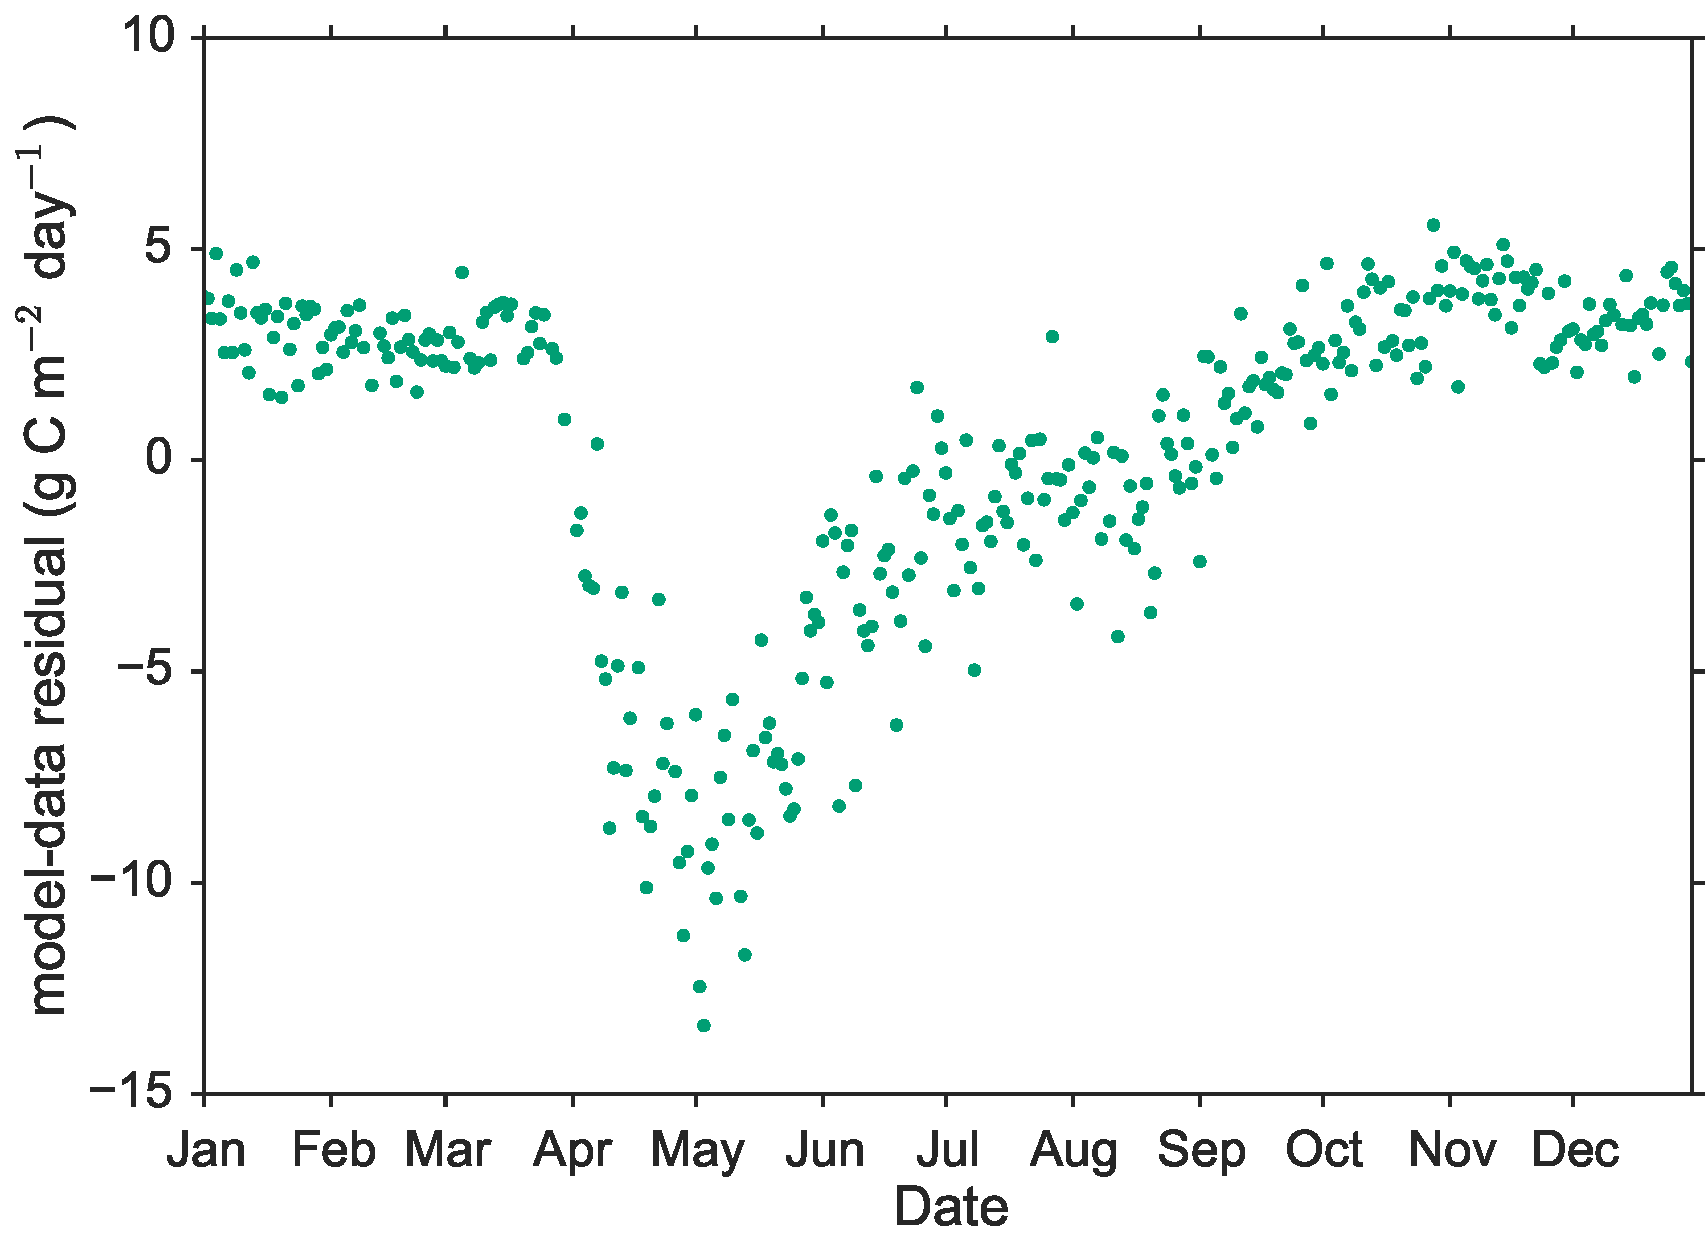
\includegraphics[width=\textwidth]{Amoddat_resid.pdf}
        \caption{Experiment A}
        \label{fig:Amoddat_resid}
    \end{subfigure}
    \begin{subfigure}[b]{0.49\textwidth}
        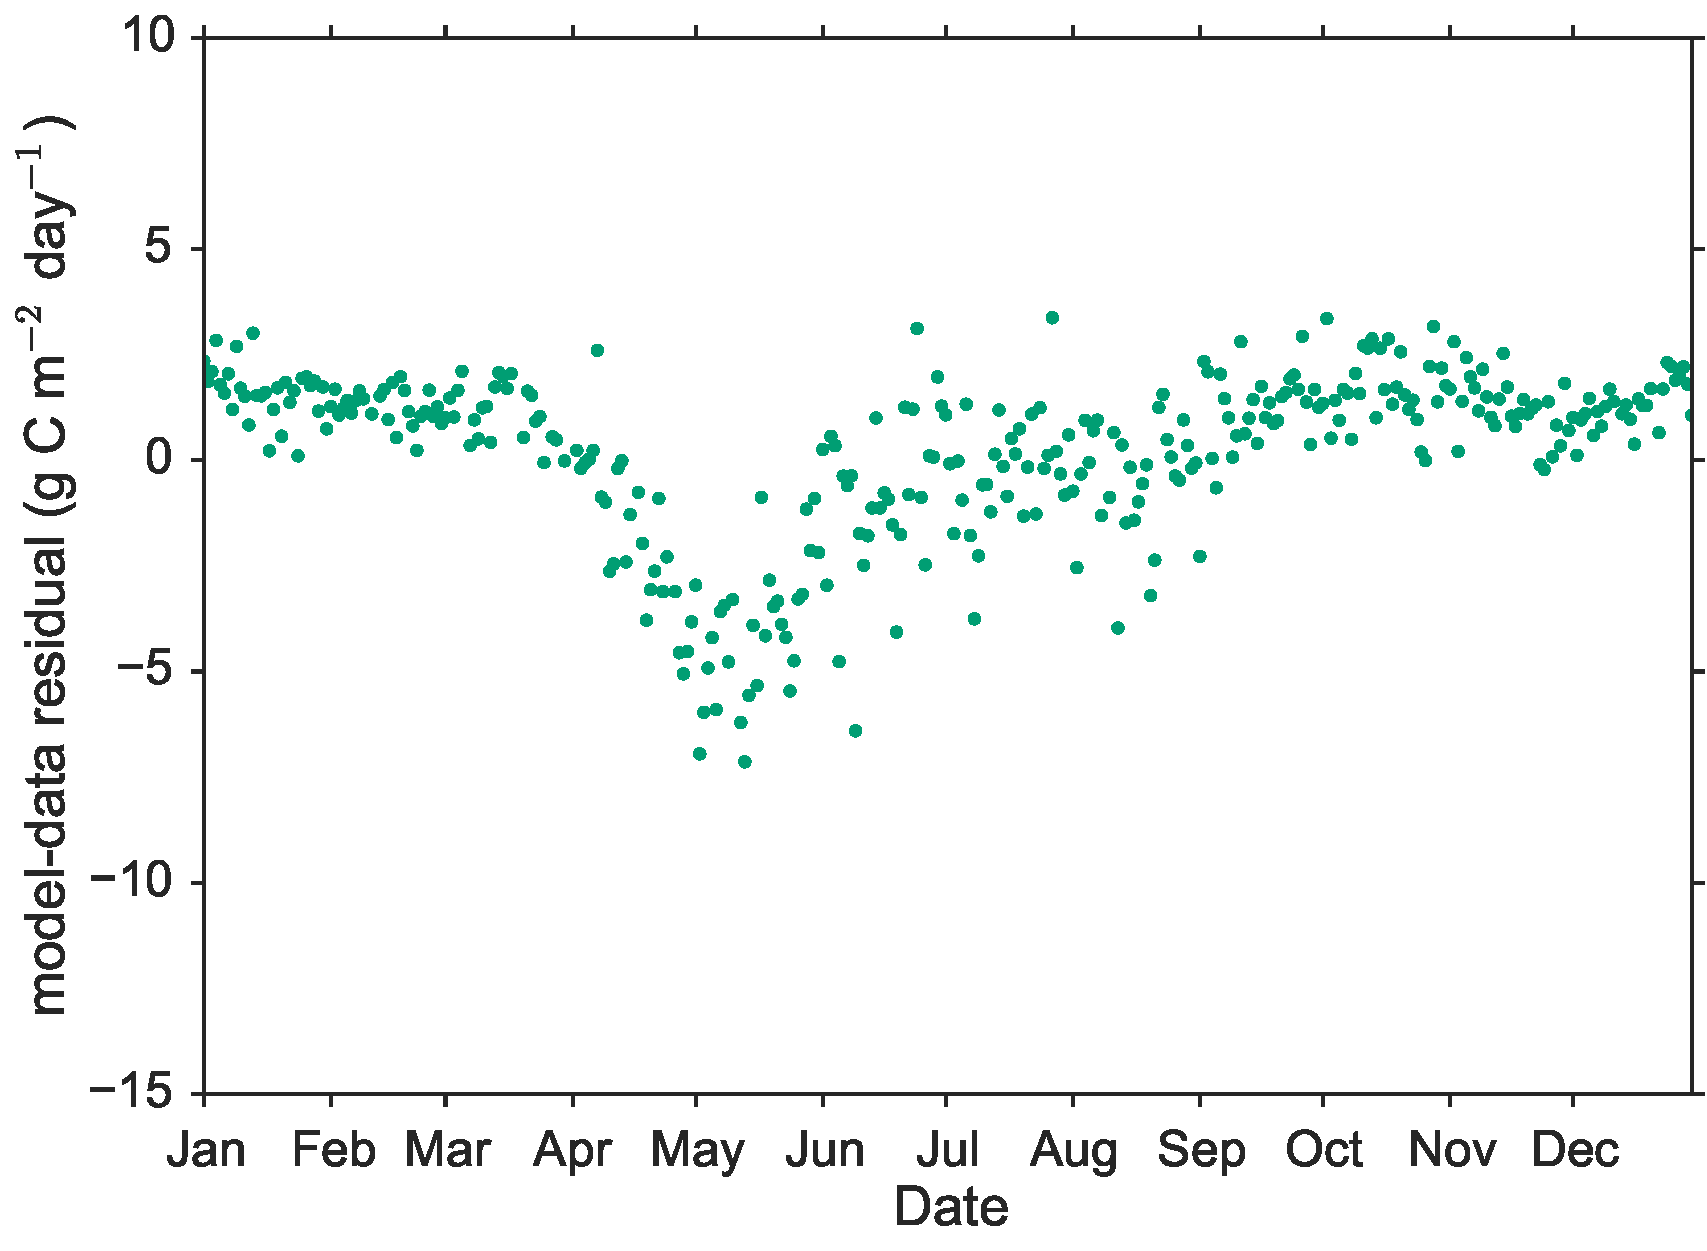
\includegraphics[width=\textwidth]{Bmoddat_resid.pdf}
        \caption{Experiment B}
        \label{fig:Bmoddat_resid}
    \end{subfigure}
    \begin{subfigure}[b]{0.49\textwidth}
        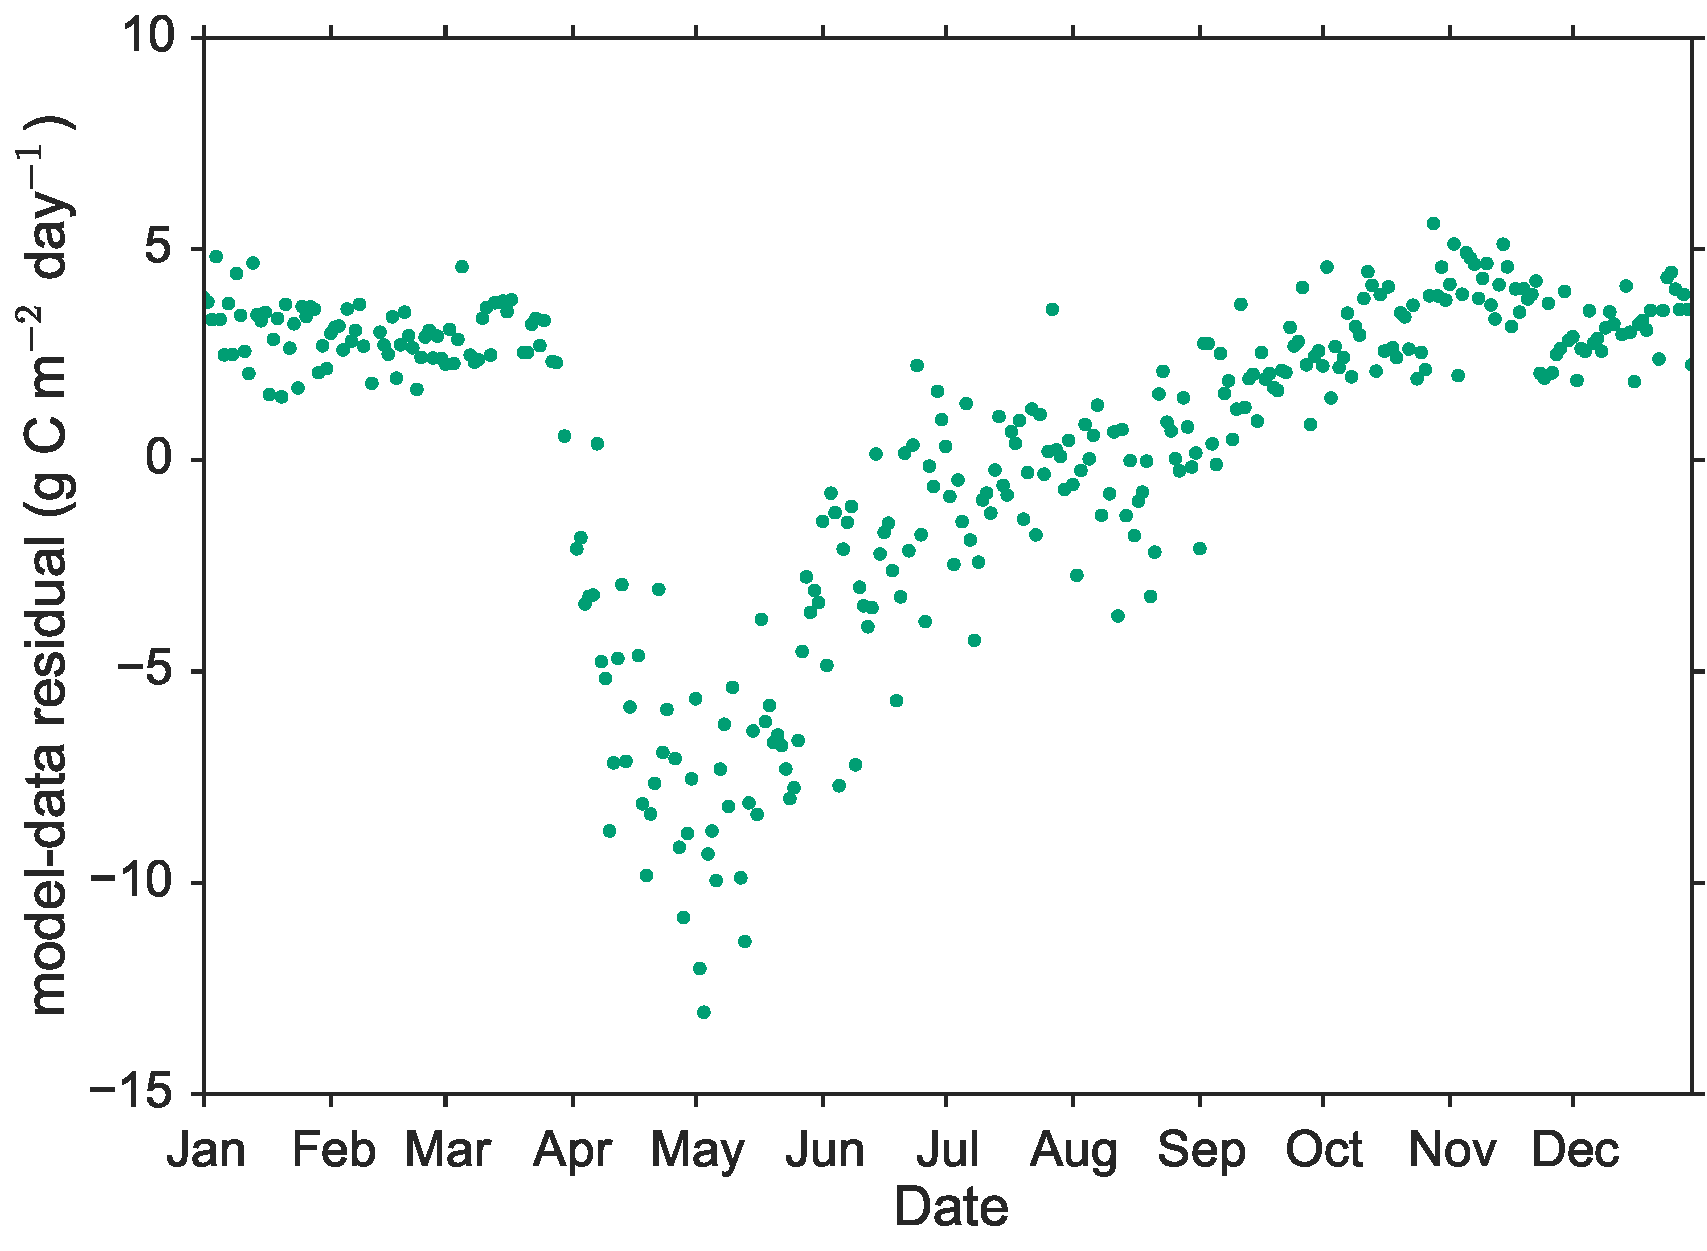
\includegraphics[width=\textwidth]{Cmoddat_resid.pdf}
        \caption{Experiment C}
        \label{fig:Cmoddat_resid}
    \end{subfigure}
    \begin{subfigure}[b]{0.49\textwidth}
        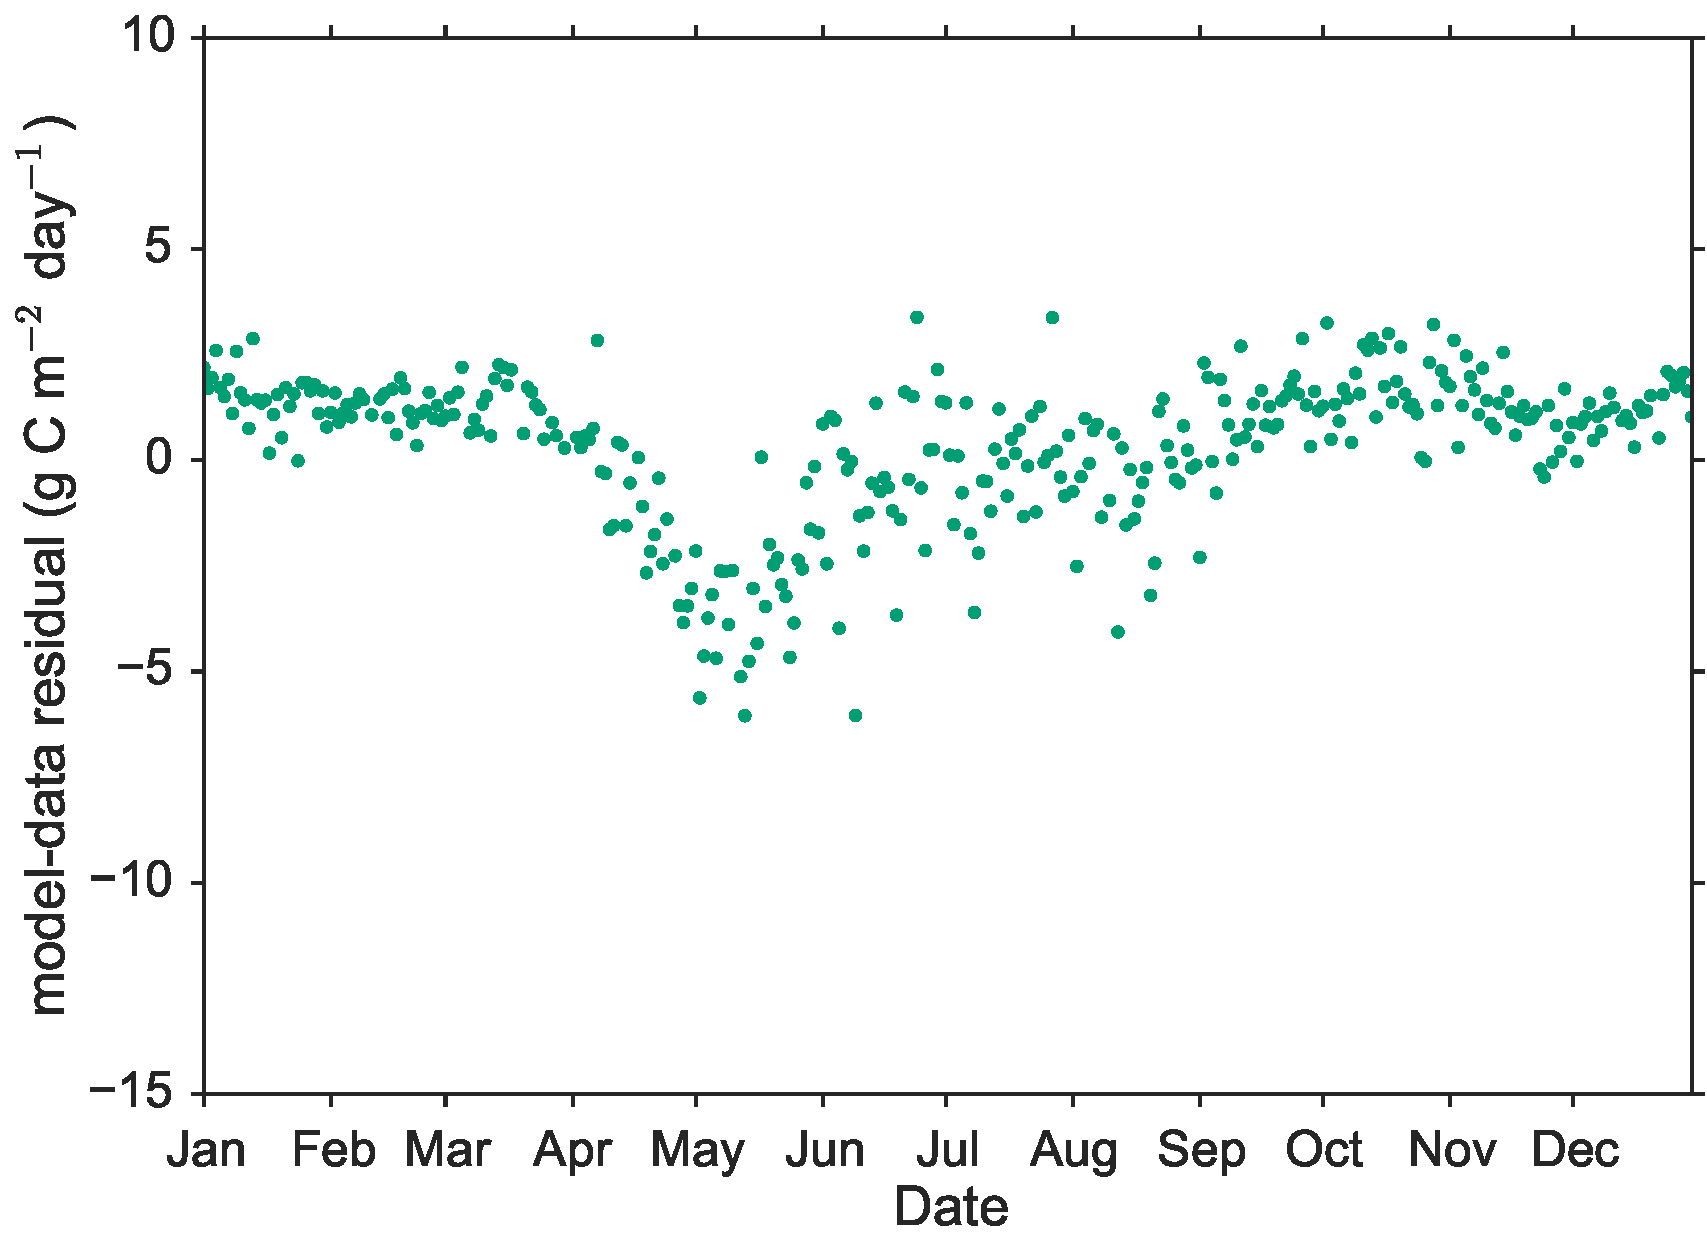
\includegraphics[width=\textwidth]{Dmoddat_resid.pdf}
        \caption{Experiment D}
        \label{fig:Dmoddat_resid}
    \end{subfigure}
    \caption{Net ecosystem exchange model-data differences for the four experiments. Here each point corresponds to the mean model-data difference for that day of the year over the 14 year model forecast (Jan 2000 - Dec 2013).}\label{fig:broke4dvar}
\end{figure}


\section{Field work} \label{sec:fieldwork}

In the last monitoring report it was discussed that a field work campaign had been undertaken to measure Leaf Area Index (LAI) at the Alice Holt flux site, using three different methods. These measurements were taken along three transects capturing both thinned and unthinned sides of the forest. Since completing the last report I have completed this fieldwork campaign and am now beginning to process the collected data.

I have also conducted a biomass survey of the Alice Holt flux site. This survey used the Point-Centred Quarters Method (PCQM) \citep{dahdouh2006empirical}. I have sampled along the three established transects. This will allow us to determine an estimate of the woody biomass for both sides of the forest. The observations that have been taken on the PhD are shown in Table~\ref{table:obs}. 

These observations will be used in the third results chapter of the thesis. We plan to use all observations that I have made with the available observations of NEE for the thinned and unthinned sides of the forest (partitioned using a flux footprint model) for data assimilation. Two versions of the DALEC2 model will be parameterised (for the thinned and unthinned sides of the forest). This will allow us to see if there is a difference between the optimised parameters for the thinned/unthinned versions of DALEC2. We will test if by just assimilating NEE we can pick out a difference in LAI between the two sides. 

We will investigate the effect of the disturbance further by parameterising DALEC2 for the thinned section of the forest both before and after the thinning occurred using the record of partitioned NEE observations. This will again allow us to see if the optimised parameters are consistent with the known changes to the forest ecosystem. From work already carried out at Forest Research it has been noted that there is no significant change in NEE between the thinned and unthinned sides of the forest, when considering only the flux towers partitioned record of NEE measurements \citep{wilkinson2016}. These experiments will hopefully allow us to answer questions we currently have about the effect of disturbance, for example:
\begin{itemize}
\item Do we see evidence that the understory and remaining dominant trees are compensating for the removed trees in the thinned section of the forest by demonstrating increased Gross Primary Productivity (GPP), as a result of reduced competition and higher light availability?
\item Is heterotrophic respiration from the soil reduced for the thinned section of forest meaning that the NEE remains similar to that of the unthinned section of forest?
\end{itemize}  
We hope that this work will form the basis for the next paper.
\begin{table}[ht] 
\begin{center}
	\begin{tabularx}{\textwidth}{| l | X | X |}
	\hline
	Observation & Method & Number of observations \\ \hline
	LAI & Ceptometer \citep{fassnacht1994comparison} & 435 \\ \hline
	LAI & Hemispherical photographs \citep{Jonckheere2004} & 89  \\ \hline
	LAI & Litter traps \citep{kimmins1973some} & 6 points measured throughout the season \\ \hline
	Woody biomass & PCQM \citep{dahdouh2006empirical} & 114  \\ 
	\hline
	\end{tabularx}
	\caption{Observations taken during the PhD at the Alice Holt research forest.}
	\label{table:obs}
\end{center} 
\end{table}

\begin{figure}[!h]
\centering
\begin{subfigure}{.5\textwidth}
  \centering
  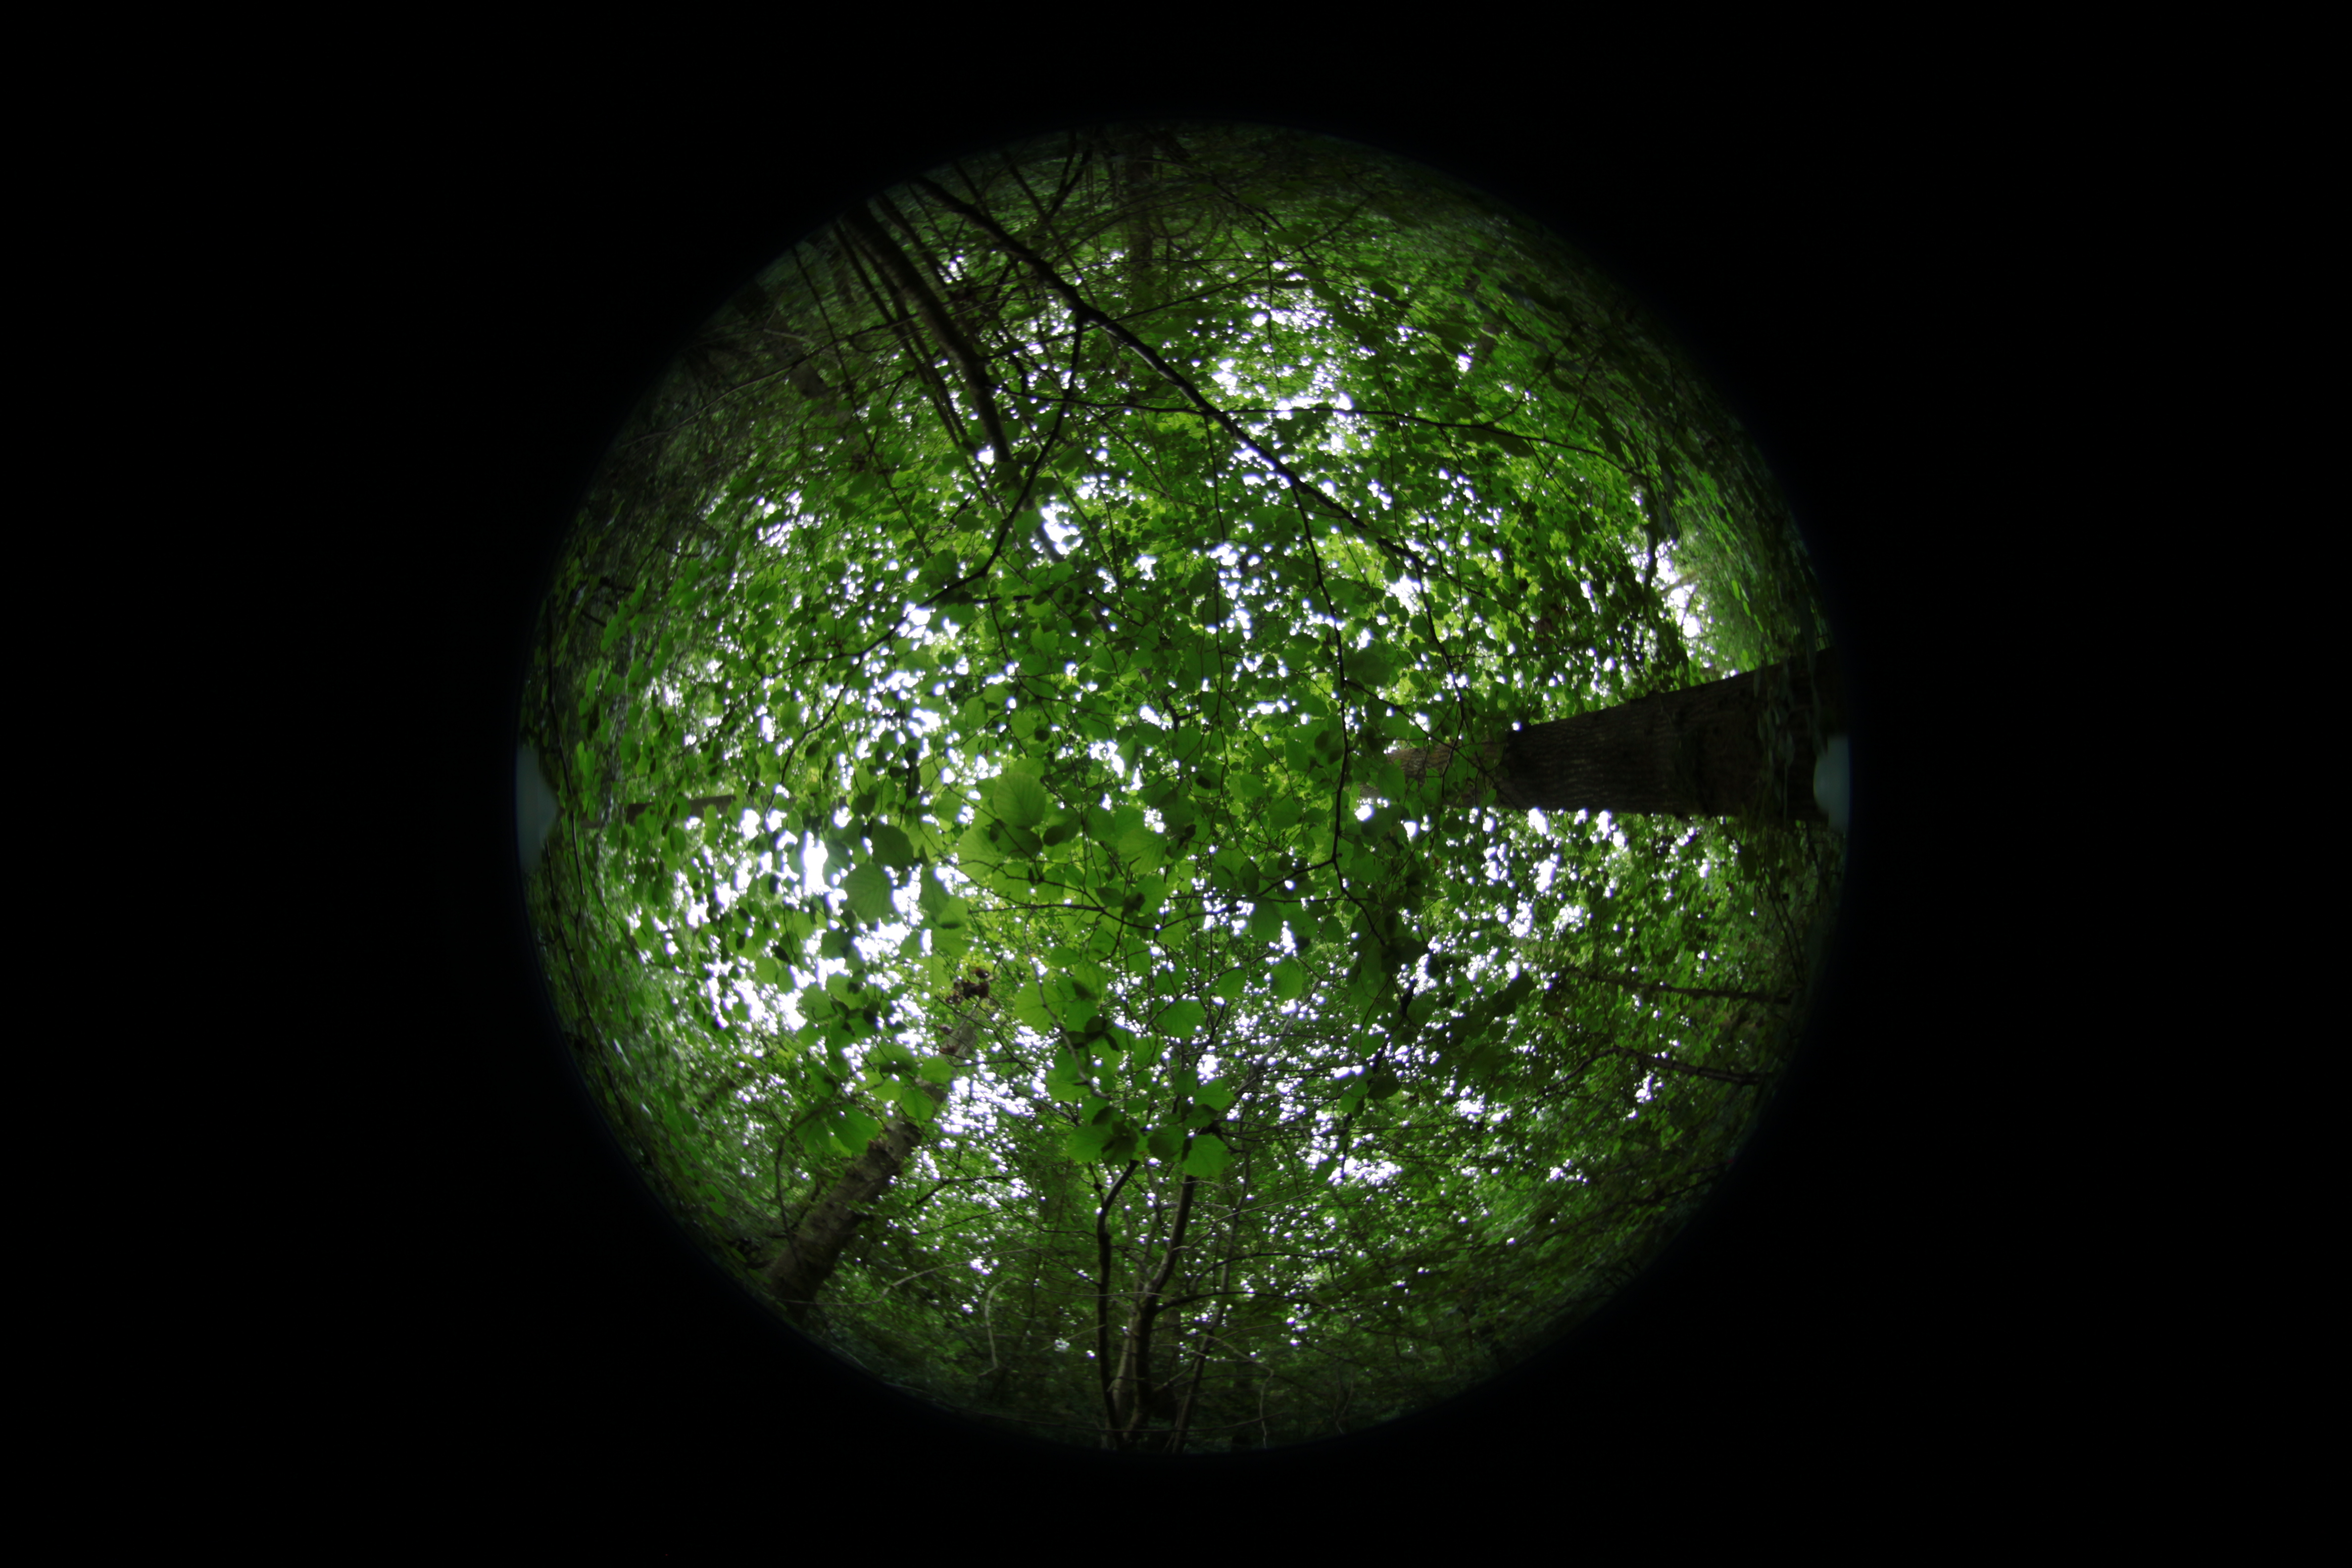
\includegraphics[width=.7\linewidth]{043exp2.jpg}
  \caption{Unthinned}
  \label{fig:sub1}
\end{subfigure}%
\begin{subfigure}{.5\textwidth}
  \centering
  \includegraphics[width=.7\linewidth]{252exp1.jpg}
  \caption{Thinned}
  \label{fig:sub2}
\end{subfigure}
\caption{Hemispherical photographs from the Alice Holt flux site showing the difference between the thinned and unthinned sides of the forest.}
\label{fig:hemiphotos}
\end{figure}

\section{Observability and information content}

A first draft of the second results chapter of the thesis on observability and information content for the DALEC2 ecosystem carbon model is close to completion. In this work we consider:
\begin{itemize}
\item The observability of the system for DALEC1 and DALEC2 with the available observations. This will allow us to see if we can find a unique analysis with the observational information alone.
\item The analytic information content in carbon balance observations for evergreen ecosystems with DALEC1 and how this information content varies over a time window.
\item The numerical information content in observations for DALEC2 for both evergreen and deciduous ecosystems over a time window.
\item The effect of including error correlations on the information content in observations.
\end{itemize}

We find that for both DALEC1 and DALEC2 our system is observable when assimilating observations of NEE only (providing we have enough observations of NEE) as shown in Figure~\ref{fig:hmat}. This means that we have enough information from observations of NEE alone to find a locally unique analysis state over a specific assimilation window with no background term \citep{zou1992incomplete}. In practice a background term is typically included in the cost function for 4D-Var data assimilation which regularises the problem and means that we always have a unique solution.

\begin{figure}
  \centering
  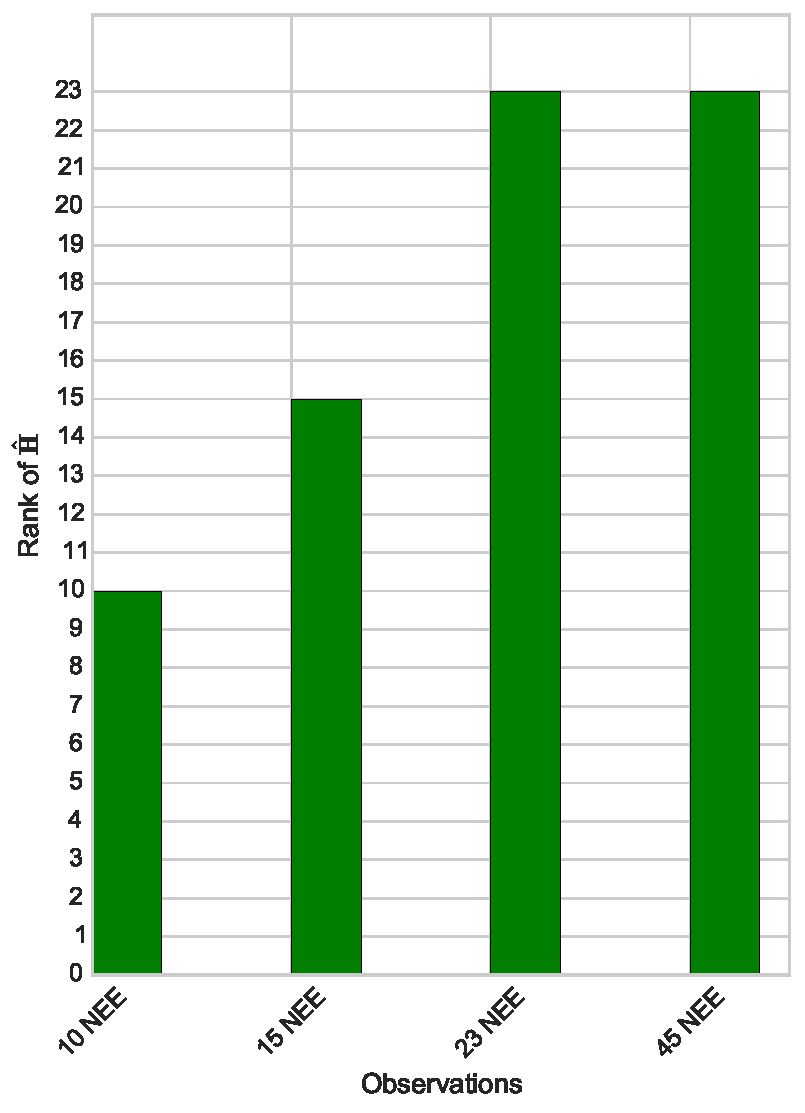
\includegraphics[width=0.5\linewidth]{hmat.pdf}
  \caption{Rank of the observability matrix $\hat{\textbf{H}}$ for increasing number of NEE observations over a years assimilation window. If the the rank of $\hat{\textbf{H}}$ is equal to 23 (the size of the state vector) then our system is observable and we can find a locally unique minimum of the observational part of the cost function.}
  \label{fig:hmat}
\end{figure}

We show that both analytic and numerical implementations of the information content measures (Shannon information content, degrees of freedom for signal and the sensitivity of the analysis to observations) give the same results. This gives us confidence that for DALEC2 our numerical implementation of these measures is correct. For DALEC1 we find temporal variation in information content for an evergreen ecosystem with observations made at times with higher temperatures having higher information content, as discussed in previous reports. We also show that including correlations in time between observation errors reduces information content. This may explain some of the results found in the attached paper, where including correlations in time between observations of NEE improves the model forecast by reducing overfitting to the observations in the assimilation window. 

For DALEC2 we find that for an evergreen ecosystem, information content in NEE observations is most reliant on temperature. However, for a deciduous site some of the NEE observations with the highest information content come during the period of green-up. This makes physical sense as the NEE for a deciduous site is controlled by phenology much more than for an evergreen site. We again find that including time correlations between observation errors reduces information content. This work is completed and in the process of being written up.

One of the main issues with assimilating only NEE is that the measurement represents the difference between GPP and Total ecosystem Respiration (RT), with NEE = RT - GPP. This means that assimilation of NEE alone can result in the over/under-prediction of RT and GPP. We hope at the end of this results chapter to consider the assimilation of day and night time NEE by using a modified observation operator in the 4D-Var DALEC2 scheme. Here night time NEE is equal to RT as no GPP occurs during the night. We hope this will help us to better partition NEE between GPP and RT. We plan to investigate this using a set of twin experiments that have already been developed. If successful this will also prove helpful for the final results chapter investigating the effect of disturbance on the Alice Holt research forest.   

\section{Professional and Academic Development}

\subsection{Masters Courses}
\begin{itemize}
\item MAMB10 (Data Assimilation) - 85\%
\item MAMNSO (Numerical Solutions to Ordinary Differential Equations) - 79\%
\item MTMG02 (Atmospheric Physics) - 66\%
\item MTMG49 (Boundary Layer) - 72\%
\item MTMD01 (Environmental Data Visualization) - 78\%
\item MTMD02 (Operational Data Assimilation) - 70\%
\end{itemize}

\subsection{Transferable Skills}

During my PhD I have taken part in the following courses, workshops and activities:
\begin{itemize}
\item 28/01/2014 - Basic Statistics Refresher - RRDP

\item 31/03/2014-01/04/2014 - Land Data Assimilation workshop at UCL - ESA

\item 23/04/2014-25/03/2014 - Correlated Observation Errors in Data Assimilation Workshop - ESA

\item 13/05/2014 - Social Media - Bloggs, Twitter and Your Online Presence - RRDP

\item 29/05/2014 - How to Write a Paper - RRDP

\item 25/06/2014-26/06/2014 - Software Carpentry Course - Git and Python

\item 10/07/2014-11/07/2014 - Forest Research - Helped with field work LiDAR

\item 21/07/2014-01/08/2014 - Fluxcourse Summer School - University of Colorado

\item 29/09/2014-03/10/2014 - NERC course - Software Development for Environmental Scientists Level 1

\item 08/10/2014-10/10/2014 - Environment YES - NERC ``dragon's den" type competition at Syngenta, Jesops Hill

\item 17/12/2014 - Presentation at Maths for Planet Earth Industry day

\item 24/02/2015 - Reading Soil Centre Workshop - What can Land Surface Models do for you?

\item 23/03/2015-27-03/2015 - NERC course - Software Development for Environmental Scientists Level 2

\item 11/03/2015 - Quo Vadis presentation

\item 08/09/2015-11/09/2015 - RSPSoc conference University of Southampton - Presented a poster

\item 24/09/2015 - Department poster presentation - Received an honourable mention for poster on ``Understanding the information content in observations of forest carbon balance"

\item 02/11/2015-03/11/2015 - BES Ecosystems and Climate Change Mitigation Conference, Charles Darwin House, London - Presented a poster

\item 02/12/2015 - RMetS SE centre meeting, Reading Town Hall - Invited to give a presentation after receiving honourable mention at the department poster presentation

\item 20/01/2016 - Submitting your thesis electronically: what you need to know - RRDP

\item 03/02/2016 - Open access and research data - RRDP

\item 12/02/2016 - How to write a thesis - RRDP

\item 15/03/2016 - How will employers interview you? - RRDP

\item 17/04/2016-22/04/2016 - EGU General Assembly, Vienna - Gave an oral presentation in the BG2.8 working group ``Developments in terrestrial biogeochemical models using model-data integration"

\begin{figure}[!ht]
    \centering
    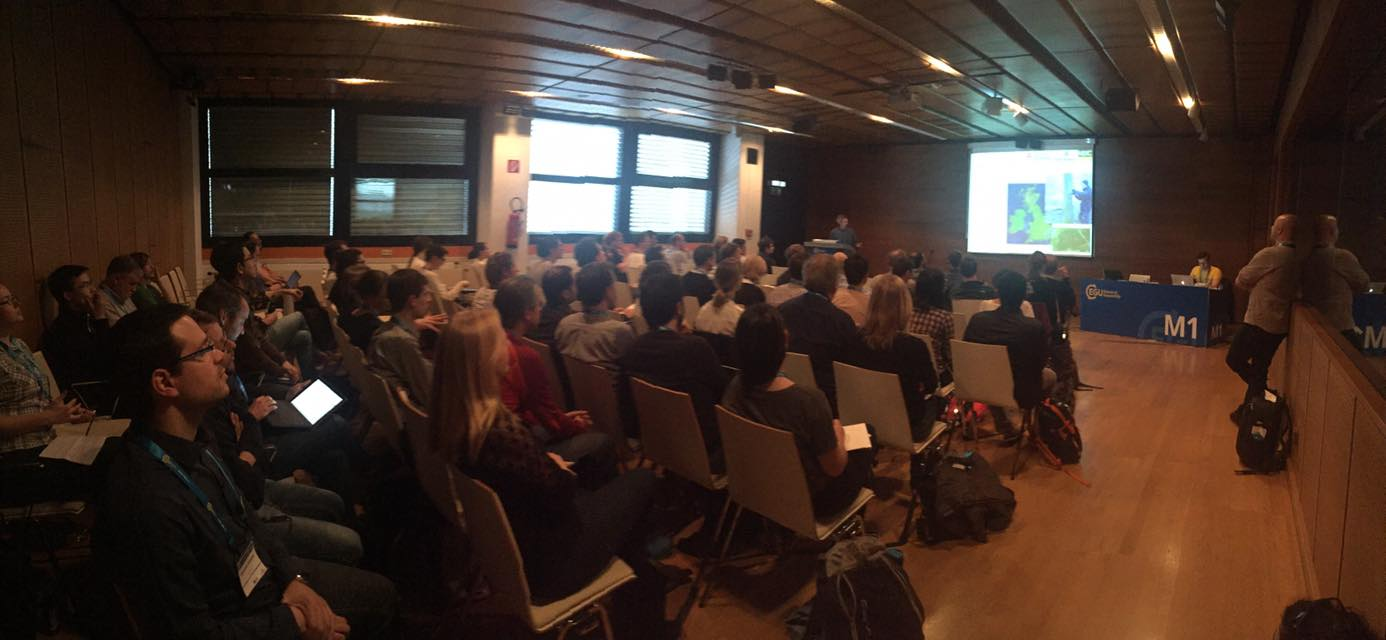
\includegraphics[width=.4\textwidth]{egu2.jpg}
    \caption{Presenting at EGU}
    \label{fig:egu}
\end{figure}

\item 12/05/2016 - Three minute thesis, Graduate School - Competed in the heats for the 3 minute thesis competition and progressed to the final at the Doctoral Research Conference

\item 23/06/2016 - Participated in the three minute thesis final at the doctoral research conference Reading
\end{itemize}



\subsection{Demonstrating}
During my PhD I have helped demonstrate on the following courses:
\begin{itemize}
\item 15/09/2014-1909/2014 - NERC Data assimilation for environmental scientists training course

\item 16/02/2015-20/02/2015 - NERC Software Development for Environmental Scientists Level 1

\item 20/04/2015-23/04/2015 - MT26E Surface Energy Exchange Practicals
\end{itemize}


\begin{table}[ht] 
\begin{center}
	\begin{tabularx}{\textwidth}{| l | X | X | X | X |}
	\hline
	Experiment & Uncorrelated prior errors, $\textbf{B}_{diag}$ & Uncorrelated observation errors, $\hat{\mathbf{R}}_{diag}$ & Correlated prior errors, $\textbf{B}_{corr}$ &
	Correlation observation errors, $\hat{\mathbf{R}}_{corr}$ \\ \hline
	A & $\times$ & $\times$ & & \\ \hline
	B & & $\times$ & $\times$ & \\ \hline
	C & $\times$ & & & $\times$ \\ \hline
	D & & & $\times$ & $\times$ \\ 
	\hline
	\end{tabularx}
	\caption{The combination of error covariance matrices used in each data assimilation experiment. $\textbf{B}_{diag}$ and $\hat{\mathbf{R}}_{diag}$ are the diagonal background and observation error covariance matrices, with no correlations and $\textbf{B}_{corr}$ and $\hat{\mathbf{R}}_{corr}$ are the background and observation error covariance matrices including correlations.}
	\label{table:exps_tab}
\end{center} 
\end{table}

\bibliography{../../PhD}{}
%\bibliographystyle{plain}
\end{document}